%%%%%%%%%%%%%%%%%%%%%%%%%%%%%%
\chapter{Current techologies}

Before I started the development of the application I have done a research period to have a better overview of the current market. There are several frameworks to choose from to start developing augmented reality applications. The most used AR frameworks are Google ARCore, Apple ARKit and RealityKit, Simple CV and Unity AR Foundation.
I ended up using Apple ARKit to build my app. I've been working with iOS development for several years and I'm sure with the Swift language as well.

\section{Unity}

One of the main frameworks that we can use if we want to develope augmented reality application is Unity.
Unity is a purpose-build framework for augmented reality development. It's key feature is that with the framework developer can easily deploy it's product across multiple mobile and wearable AR devices. It includes core features from ARKit(Apple), ARCore(Google) and HoloLens(Microsoft) as well unique features.

AR Foundation which is the recommended framework for Unity development there are several features what the developers can use like:
\begin{itemize}
    \item Device tracking
    \item Raycast
    \item Plane detection
    \item Gestures
    \item Face tracking
\end{itemize}

\section{Apple ARKit and RealityKit}

Apple ARKit and RealityKit are two powerful technologies developed by Apple that enable the creation of immersive augmented reality experiences on iOS devices. ARKit is a software framework that provides developers with the tools and resources they need to build augmented reality apps for iPhones and iPads. It allows developers to easily place virtual objects in the real world, track the user's position and orientation, and integrate real-time camera data to create realistic and interactive experiences.

On the other hand, RealityKit is a high-level framework that makes it easy for developers to create 3D content and build AR experiences without requiring extensive knowledge of 3D graphics or game engine programming. RealityKit includes features such as physics simulations, animations, and spatial audio, which can be used to create highly immersive AR experiences.

Together, ARKit and RealityKit provide developers with a comprehensive set of tools for building augmented reality experiences on iOS devices. With these technologies, developers can create innovative and engaging apps that allow users to interact with virtual objects in the real world, opening up new possibilities for gaming, education, and more.

\begin{figure}[!ht]
    \centering
    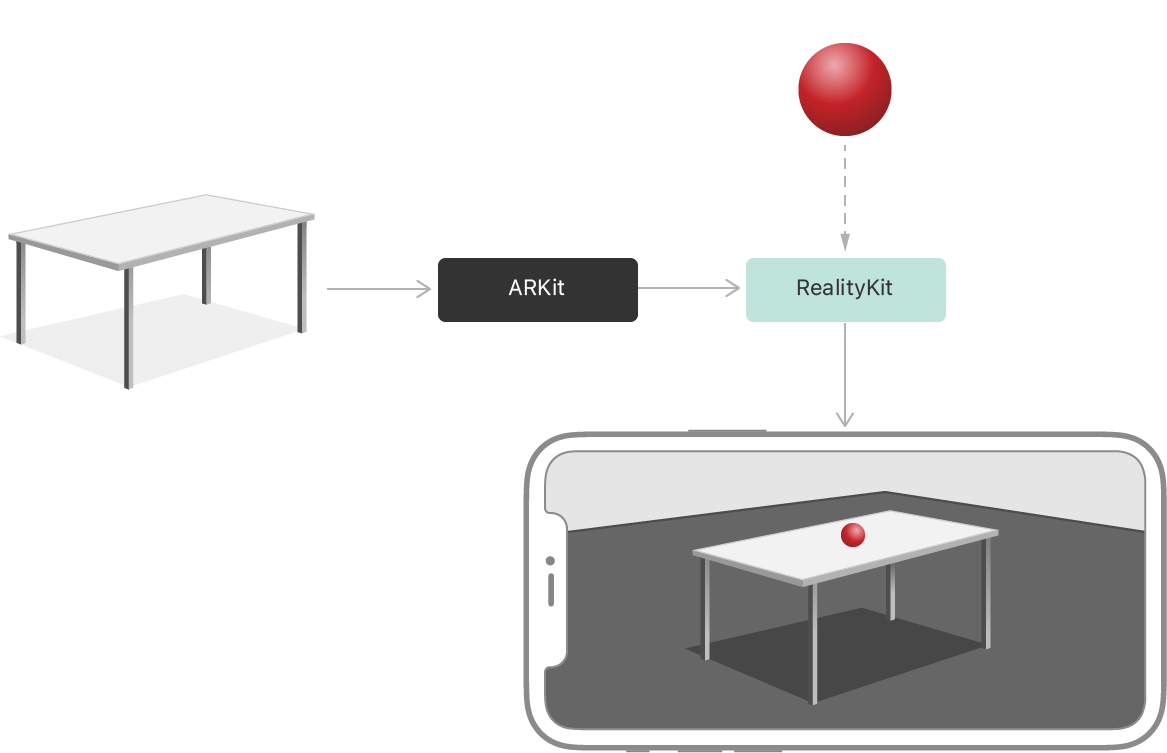
\includegraphics[width=150mm]{../images/realitykit.png}
    % \includegraphics[width=150mm, keepaspectratio]{figures/TeXnicCenter.png}
    \caption{RealityKit and ARKit usage.}
    \label{fig:TexnicCenter}
\end{figure}



RealityKit’s features:
\begin{itemize}
    \item Rendering: RealityKit offers a powerful new physically-based renderer built on top of Metal, which is fully optimized for all Apple devices.

    \item Animation: It has built-in support for Skeletal animation and Transform-based animation. So, if you want, you can animate anithing or you can move, scale and rotate objects with various easing functions.

    \item Physics: With a powerful physics engine, RealityKit lets you adjust real-world physics properties like mass, drag and restitution, allowing you to fine-tune collisions.

    \item Audio: Spacial audio understanding and automatic listener configuration let you attach sound effects to 3D objects. You can then track those sounds, making them sound realistic based on their position in the real world.

    \item ECS: From a coding perspective, RealityKit enforces the Entity Component System design pattern to build objects within the world.

    \item Synchronization: The framework has built-in support for networking, designed for collaborative experiences. It even offers automatic synchronization of entities between multiple clients.
\end{itemize}
